\chapter{Work Packages}
\label{sec:schedule}
\begin{figure}[H]
    \centering
    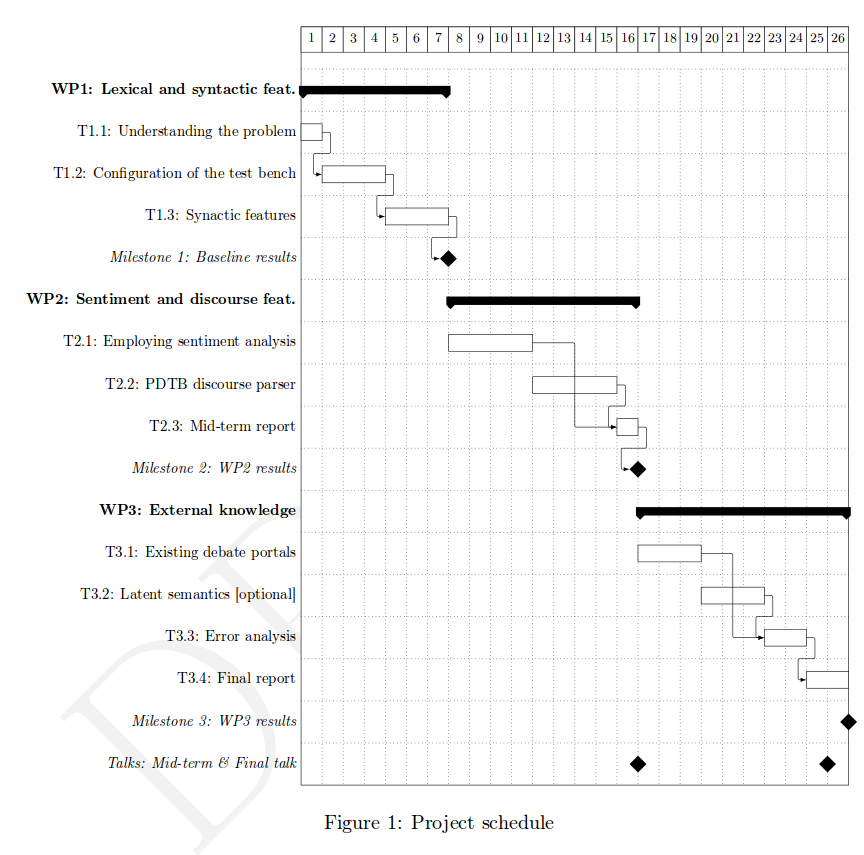
\includegraphics[width=0.9\textwidth]{fig/schedule.png}
    \caption[Short caption]{Project schedule}
    \label{fig:schedule}
\end{figure}
\chapter{DKPro Core Overview}
\begin{figure}[ht]
    \centering
    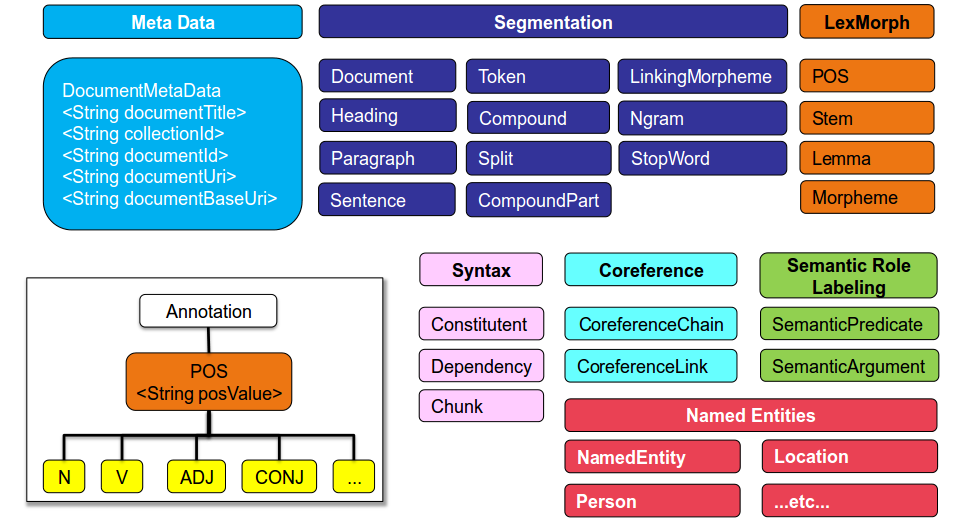
\includegraphics[width=1\textwidth]{fig/dkpro-overview.png}
    \caption[Short caption]{DKPro Type System}
    \label{fig:dkpro-overview}
\end{figure}
\label{sec:dkpro overview}

\chapter{Xmi Files - Example}
\label{sec:xmi}
\begin{figure}[H]
    \centering
    
\includegraphics[width=0.9\textwidth]{fig/xmifile.png}
    \caption[Short caption]{Example of XMI file}
    \label{fig:dkpro-overview}
\end{figure}

\chapter{Binary Classification}
\label{sec:bincla}
\textbf{Cross-Validation and Train-Test Scenarios}
\\
First, we should keep in mind that those two scenarios can also be evaluated for other problems than binary classification. For the train-test scenario, we simply have two sets, the \emph{training set} that will be used to train our model and the test set for making the predictions. In the n folds cross-validation scenario we split our data in n folds, one of the fold will be the test set and the n-1 others will form the training set. The predictions are evaluated n times.
\\
\\
\textbf{Basic definitions}
\\
Suppose we have to classes (to keep the report example, P1 and P2), one called \emph{positive} (here P1) and the other \emph{negative}\footnote{This designation come from the fact that binary classification is usually used in epidemiology (The patient is sick or not)}. Then we run our algorithm (with a cross-validation or a train-test scenario) and we can report four cases:
\begin{itemize}
  \item \textit{True Positive (TP)}: A P1 instance was recognized as P1.
  \item \textit{True Negative (TN)}: A P2 instance was recognized as P2. 
  \item \textit{False Positive (FP)}: A P2 instance was recognized as P1. 
  \item \textit{False Negative (FN)}: A P1 instance was recognized as P2. 
\end{itemize}
\\
\\
\textbf{Confusion Matrix}
\\
It's a 2 by 2 matrix that summarizes the prediction results as follow:
\\
\noindent
\renewcommand\arraystretch{1.5}
\setlength\tabcolsep{0pt}
\begin{tabular}{c >{\bfseries}r @{\hspace{0.7em}}c @{\hspace{0.4em}}c @{\hspace{0.7em}}l}
  \centering
  \multirow{10}{*}{\parbox{1.1cm}{\bfseries\raggedleft actual\\ value}} & 
    & \multicolumn{2}{c}{\bfseries Prediction outcome} & \\
  & & \bfseries P1 & \bfseries P2 & \bfseries total \\
  & P1 & \MyBox{True}{Positive} & \MyBox{False}{Negative} & P$'$ \\[2.4em]
  & P2 & \MyBox{False}{Positive} & \MyBox{True}{Negative} & N$'$ \\
  & total & P & N &
\end{tabular}
\\
\\
\\
\textbf{Statistical measures calculated from the Confusion Matrix}
\\

\textit{Sensitivity}: Sensitivity (also called the true positive rate, or the recall rate in some fields) measures the proportion of actual positives which are correctly identified as such (here the percentage of P1 instances which are correctly identified as persuasive). The formula is:
\begin{equation*}
Sensitivity = \frac{TP}{TP + FN}
\end{equation*}
\\

\textit{Specificity}:  Specificity (sometimes called the true negative rate) measures the proportion of negatives which are correctly identified as such (here the percentage of P2 instances which are correctly identified as non persuasive). The formula is:
\begin{equation*}
Specificity = \frac{TN}{TN + FP}
\end{equation*}
\\

\textit{Accuracy}: In binary classification, the accuracy is the proportion of true results (both true positives and true negatives). The formula is:
\begin{equation*}
Accuracy = \frac{TN + TP}{TN + TP + FN + FP}
\end{equation*}
\\

\textit{Macro F-measure}: In case of high biased in our data (for example 99\% of negative instances and 1\% of positive instances), the accuracy is not a relevant metric anymore. Indeed a classifier that foolishly predict all the instances as negative will have, an accuracy of 99\%. Thus, we introduce the macro F-measure which can be seen as the harmonic mean of precision and sensitivity. The formula is:
\begin{equation*}
Fm = \frac{2 TP}{2 TP + FN + FP}
\end{equation*}